\documentclass[]{style}
\usepackage{amsmath,amssymb}
\usepackage{graphicx}
\usepackage{booktabs}
\usepackage{array}
\usepackage{tabularx}
\usepackage{enumitem}
\graphicspath{{bench/}}

\title{\fontsize{0.6cm}{0.72cm}\selectfont Maintaining a Living Virtual Cell Benchmark\\[0.3cm] with Item Response Theory}

\author[1]{Author One}
\author[1]{Author Two}
\affiliation[1]{Northwestern University}

\abstract{Current virtual cell benchmarks face two major problems. First, they score
models mainly by raw accuracy or average error, even though test cases differ greatly in
difficulty. Second, a fixed benchmark loses value over time: test cases become too easy as
the field moves forward, and they become less reliable once they are widely known and enter
training data. We address both problems with a benchmark that assigns every test case a
measured difficulty, as standardized tests such as the SAT and GRE do. The current release
aggregates fourteen annotation panels drawn from seven public atlases, including Tabula
Sapiens v2 and the scBaseCount repository, and fifteen public perturbation screens, about
110 million cells in all, into 424,478 cell-type annotation items covering 299 cell-type
labels and 88,164 perturbation items covering roughly 10,000 gene targets, 500 compounds and
90 cytokines in more than 450 cell lines, donors and culture conditions. We evaluate [N]
models on it, from principal components and ridge regression to scVI and scGen.
Difficulties are estimated with a one-parameter item response model from a pool of
deliberately simple models, so the scale is anchored to methods that cannot have memorized
the test data. We report the resulting difficulty distributions, the abilities of every
model on each component, and the fraction of items that are already uninformative for the
evaluated models, which fixes the rate at which new hard items must be written.}

\begin{document}
\maketitle

% ---------------------------------------------------------------------------
\section{Introduction}
\label{sec:intro}

To be filled.

% ---------------------------------------------------------------------------
\section{Dataset Composition and Statistics}
\label{sec:data}

We call every test case an \emph{item}.
Depending on the task, an item could be one cell or one experimental condition.
Each item carries a difficulty, and each model an ability, both estimated from which items
the model passes. The bank has two components with different items
but the same pass/fail response format.

\paragraph{Component A: representation.}
An item is one cell. A model maps a cell's expression profile to a vector. The response is
whether a multinomial logistic regression, trained once on the vectors of a separate
training panel with fixed settings, assigns the cell its annotated type. The classifier is
identical for every model, so a difference in responses is a difference in embeddings.

\paragraph{Component B: perturbation.}
An item is one experimental condition: a perturbation applied in one context.
A perturbation is a knockout or knockdown target gene, a compound, or a cytokine.
A context is a cell line, a donor, or a cell type.
When a dataset contains more than one kind of context, the context is their combination,
for example a donor and a cell type.
The cells of a condition are replicates, not items; the measured response of a condition is
the mean log-normalized expression of its cells minus that of its matched control cells.
A model predicts this response for conditions it has not been trained on.
We score a prediction by its Pearson correlation with the measured response over the 2,000
most variable genes, and the item is passed when that correlation exceeds the context-mean
baseline. We call this reference the \emph{mean shift}, and it is chosen on purpose. Recent
benchmarks \citep{systema,perturbench,ahlmann2025} found that this average matches deep
models on standard metrics, because much of any response is shared across perturbations; a
pass therefore credits the perturbation-specific part of a prediction and not the part
every perturbation shares.

\paragraph{Sources.}
Component A draws on seven sources: Tabula Sapiens v2 \citep{tabulasapiens2}; four curated
atlases from CELLxGENE, namely the Hao 2021 PBMC reference \citep{hao2021}, the adult heart
atlas \citep{litvinukova2020}, the Human Lung Cell Atlas core \citep{sikkema2023} and the
cross-tissue immune atlas \citep{dominguezconde2022}; the Parse 10 million PBMC cytokine
atlas \citep{parsepbmc}; and scBaseCount \citep{scbasecount}, a repository of uniformly
reprocessed public single-cell submissions with machine-curated labels. Component B uses
thirteen screens from the scPerturb collection \citep{scperturb}, the Tahoe-100M drug atlas
\citep{tahoe} and the Parse cytokine atlas; see \Cref{tab:compB}. All sources are public
under CC0, CC BY or CC BY-NC licences.


\paragraph{Representation panels.}
Every annotation source is turned into one or more \emph{panels} by the same procedure.
The unit of the split is chosen first: whole donors, whole studies, or whole tissues are
held out, so that nothing is shared between the training panel and the test items and the
classifier cannot learn donor, study, or tissue identity as a stand-in for cell type. We
call each combination of context, cell type and donor a \emph{stratum}; within each stratum
we keep at most 200 training and 50 to 100 test cells and drop strata with fewer than 20
cells. Test cells whose type is absent from training are kept in the panel but not scored.
\Cref{tab:compA} lists the fourteen panels. Eleven hold out donors, which is the standard
annotation setting; three hold out whole studies or tissues, so that a type must be
recognized in a context the classifier has never seen. The HLCA and the immune atlas appear
twice, once under each split. The scBaseCount panels differ from the curated atlases in
one respect that matters below: each holds every filter-passing sample up to 200 per tissue,
between 78 and 200 samples from different public submissions, and the twelve-tissue panel
355 samples; labels are drawn from the repository's per-cell annotation, so the label
vocabulary is not uniform across samples. Two further panels were built and set aside as
floors: a Parse panel whose label is the cytokine a cell was exposed to, which no embedding
and probe answer above a few percent, and a mouse twelve-tissue scBaseCount panel with 109
label vocabularies, on which 60\% of items are passed by nothing. Six mouse single-tissue
panels were also run; this release pools human panels only. \Cref{tab:compA_ts2} in the
appendix gives the Tabula Sapiens panel by tissue.

\begin{table}[t]
\centering
\caption{Representation panels. Cell types counts the distinct labels among a panel's items;
none pass is the fraction of items that no model labels correctly; mean difficulty is on
the pooled scale of \Cref{sec:fitting}, over informative items. Panels hold out whole donors
unless marked otherwise; the held-out units, contexts and strata of every panel are listed in
\Cref{tab:compA_full}.}
\label{tab:compA}
\footnotesize
\begin{tabular}{@{}lrrrrr@{}}
\toprule
Tissue & Donors & Cell types & Training cells & Items & Strata \\
\midrule
Small Intestine & 5 & 31 & 5,684 & 1,800 & 40 \\
Spleen & 6 & 21 & 10,604 & 1,326 & 28 \\
Fat & 6 & 20 & 5,897 & 1,234 & 26 \\
Stomach & 3 & 18 & 1,252 & 1,232 & 26 \\
Large Intestine & 5 & 25 & 4,785 & 1,228 & 26 \\
Tongue & 4 & 20 & 3,040 & 1,226 & 26 \\
Lung & 4 & 28 & 10,472 & 1,220 & 25 \\
Thymus & 5 & 25 & 9,098 & 1,219 & 29 \\
Bladder & 6 & 21 & 8,776 & 1,140 & 25 \\
Lymph Node & 6 & 19 & 9,119 & 1,039 & 22 \\
Heart & 5 & 15 & 2,618 & 1,026 & 22 \\
Muscle & 5 & 22 & 5,394 & 999 & 21 \\
Bone Marrow & 6 & 20 & 7,737 & 916 & 21 \\
Vasculature & 4 & 20 & 5,223 & 844 & 18 \\
Salivary Gland & 4 & 23 & 6,501 & 679 & 15 \\
Trachea & 5 & 20 & 4,086 & 621 & 15 \\
Prostate & 3 & 12 & 2,771 & 555 & 12 \\
Blood & 9 & 18 & 11,510 & 504 & 11 \\
Mammary & 2 & 12 & 1,837 & 498 & 10 \\
Ear & 2 & 9 & 298 & 300 & 6 \\
Ovary & 3 & 9 & 2,268 & 270 & 6 \\
Testis & 1 & 8 & 0 & 150 & 3 \\
Eye & 4 & 28 & 7,045 & 0 & 0 \\
Kidney & 1 & 10 & 1,371 & 0 & 0 \\
Liver & 4 & 20 & 7,673 & 0 & 0 \\
Pancreas & 2 & 14 & 2,594 & 0 & 0 \\
Skin & 4 & 14 & 4,954 & 0 & 0 \\
Uterus & 2 & 17 & 4,193 & 0 & 0 \\
\midrule
Total & 23 & 159 & 146,800 & 20,026 & 433 \\
\bottomrule
\end{tabular}

\end{table}

\begin{table}[t]
\centering
\caption{Perturbation items by source. An item is a condition with at least 50
quality-passing cells and a matched control. Contexts are cell lines, culture conditions,
or donor and cell type pairs. Tahoe-100M conditions are compound, dose and cell line
triples; Parse conditions are cytokine, donor and cell type triples; the Replogle
genome-wide screen is the largest genetic source. Cell counts are after quality filtering.}
\label{tab:compB}
\footnotesize
\begin{tabular}{@{}llrrrr@{}}
\toprule
Dataset & Perturbation & Contexts & Perturbations & Items & Cells \\
\midrule
Tahoe-100M & compound, 3 doses & 50 & 379 & 53,972 & 95.6M \\
Parse 10M PBMC & cytokine & 215 & 90 & 13,967 & 9.6M \\
Replogle 2022, K562 genome-wide & CRISPRi & 1 & 9,326 & 9,326 & 1.97M \\
sciPlex3, Srivatsan 2020 & compound, 4 doses & 3 & 188 & 2,423 & 762k \\
Replogle 2022, K562 essential & CRISPRi & 1 & 1,832 & 1,832 & 303k \\
Nadig 2024, Jurkat & CRISPRi & 1 & 1,815 & 1,815 & 245k \\
Replogle 2022, RPE1 & CRISPRi & 1 & 1,611 & 1,611 & 225k \\
Nadig 2024, HepG2 & CRISPRi & 1 & 1,061 & 1,061 & 104k \\
McFarland 2020 & compound, 7 doses & 196 & 16 & 866 & 166k \\
Frangieh 2021 & CRISPR knockout & 3 & 229 & 669 & 216k \\
Norman 2019 & CRISPRa, single and double & 1 & 236 & 236 & 111k \\
Tian 2021, neurons & CRISPRi & 1 & 183 & 183 & 32k \\
Adamson 2016 & CRISPRi & 1 & 87 & 87 & 63k \\
Tian 2019, iPSC & CRISPRi & 1 & 81 & 81 & 29k \\
Tian 2019, neurons & CRISPRi & 1 & 35 & 35 & 8k \\
\midrule
Total & & & & 88,164 & 109.5M \\
\bottomrule
\end{tabular}
\end{table}

\paragraph{Perturbation items.}
Every screen is mapped to one schema with perturbation, target genes, modality, context,
dose, time and a control flag; cells with fewer than 500 counts or 200 detected genes are
removed; and the per-condition mean is computed in one pass over the raw count matrix. For
Tahoe-100M this pass streams 95.6 million cells from the public parquet files and reduces
them to 56,827 conditions, of which 53,972 have at least 50 cells; for Parse it streams 9.7
million cells and yields 13,967 conditions over 90 cytokines, 12 donors and 18 cell types,
each with its own PBS control. Median cells per item range from 74 for Nadig HepG2 to 1,363
for Tahoe-100M. Each item carries covariates for later analysis: cell count, an effect-size
measure, which is the Euclidean norm of the response, the target gene or the compound's
chemical structure, and dose.

\paragraph{Difficulty distributions.}
\Cref{fig:difficulty} shows the fitted difficulties. The 5th to 95th percentiles of the
informative items are $-3.5$ to $3.2$ for cells and $-3.4$ to $1.4$ for conditions, with
standard deviations of 1.9 and 1.5; the abilities of the models occupy the shaded band in
each panel. 52,890 cells, or 12\%, are labelled correctly by no model and 1,247 by every
model; 21,733 conditions, or 25\%, are passed either by every model or by none, all but 56
of them by none. In Tahoe-100M the fraction passed by none is 28\%, in Parse 24\% and in the
Tian 2021 neuronal screen 61\%; among the annotation panels it ranges from 1\% for Parse to
32\% for the twelve-tissue scBaseCount panel. On the pooled annotation scale the mean
difficulty by panel ranges from $-1.9$ for Parse to $-0.05$ for the twelve-tissue
scBaseCount panel; the six scBaseCount panels have means between $-0.9$ and $-0.05$ and
the eight curated panels between $-1.9$ and $-0.1$. On the pooled perturbation scale the
mean by dataset ranges from $-2.6$ for Norman to $+0.6$ for Tian 2021 neurons, with
Tahoe-100M at $-1.0$ and Parse at $+0.3$; the within-dataset standard deviation is about
1.5.

\paragraph{Difficulty and item covariates.}
Within the curated atlases, cell difficulty falls with the number of training cells of the
same type: Spearman $\rho$ is $-0.35$ for Tabula Sapiens, $-0.39$ for Hao, $-0.33$ and
$-0.29$ for the two HLCA panels and $-0.25$ and $-0.12$ for the two immune-atlas panels.
On the single-tissue scBaseCount panels $\rho$ is between $-0.04$ and $+0.17$, and on the
Parse panel $+0.51$; the twelve-tissue scBaseCount panel gives $-0.43$. Difficulty falls
with sequencing depth on every panel, $\rho$ between $-0.02$ and $-0.38$, most strongly on
the scBaseCount skin and lung panels. Across the pooled scale the two correlations are
$0.00$ and $-0.19$. The hardest cell types in the curated atlases are sibling immune states
such as activated versus naive CD8 T cells, gamma-delta T cells, innate lymphoid cells and
intermediate monocytes, and stromal types that share a lineage; on the scBaseCount panels
they are coarse or progenitor labels such as leukocyte, common myeloid progenitor and
granulocyte-monocyte progenitor. For conditions, difficulty rises with effect size in the
genetic screens, $\rho=+0.16$ in the genome-wide K562 screen and $+0.19$ in RPE1, and falls
with it in the compound and cytokine screens, $-0.23$ for sciPlex3, $-0.27$ for McFarland
and $-0.31$ for Parse. The continuous scores are kept so that a graded fit can be run
alongside the binary one.

\begin{figure}[t]
\centering
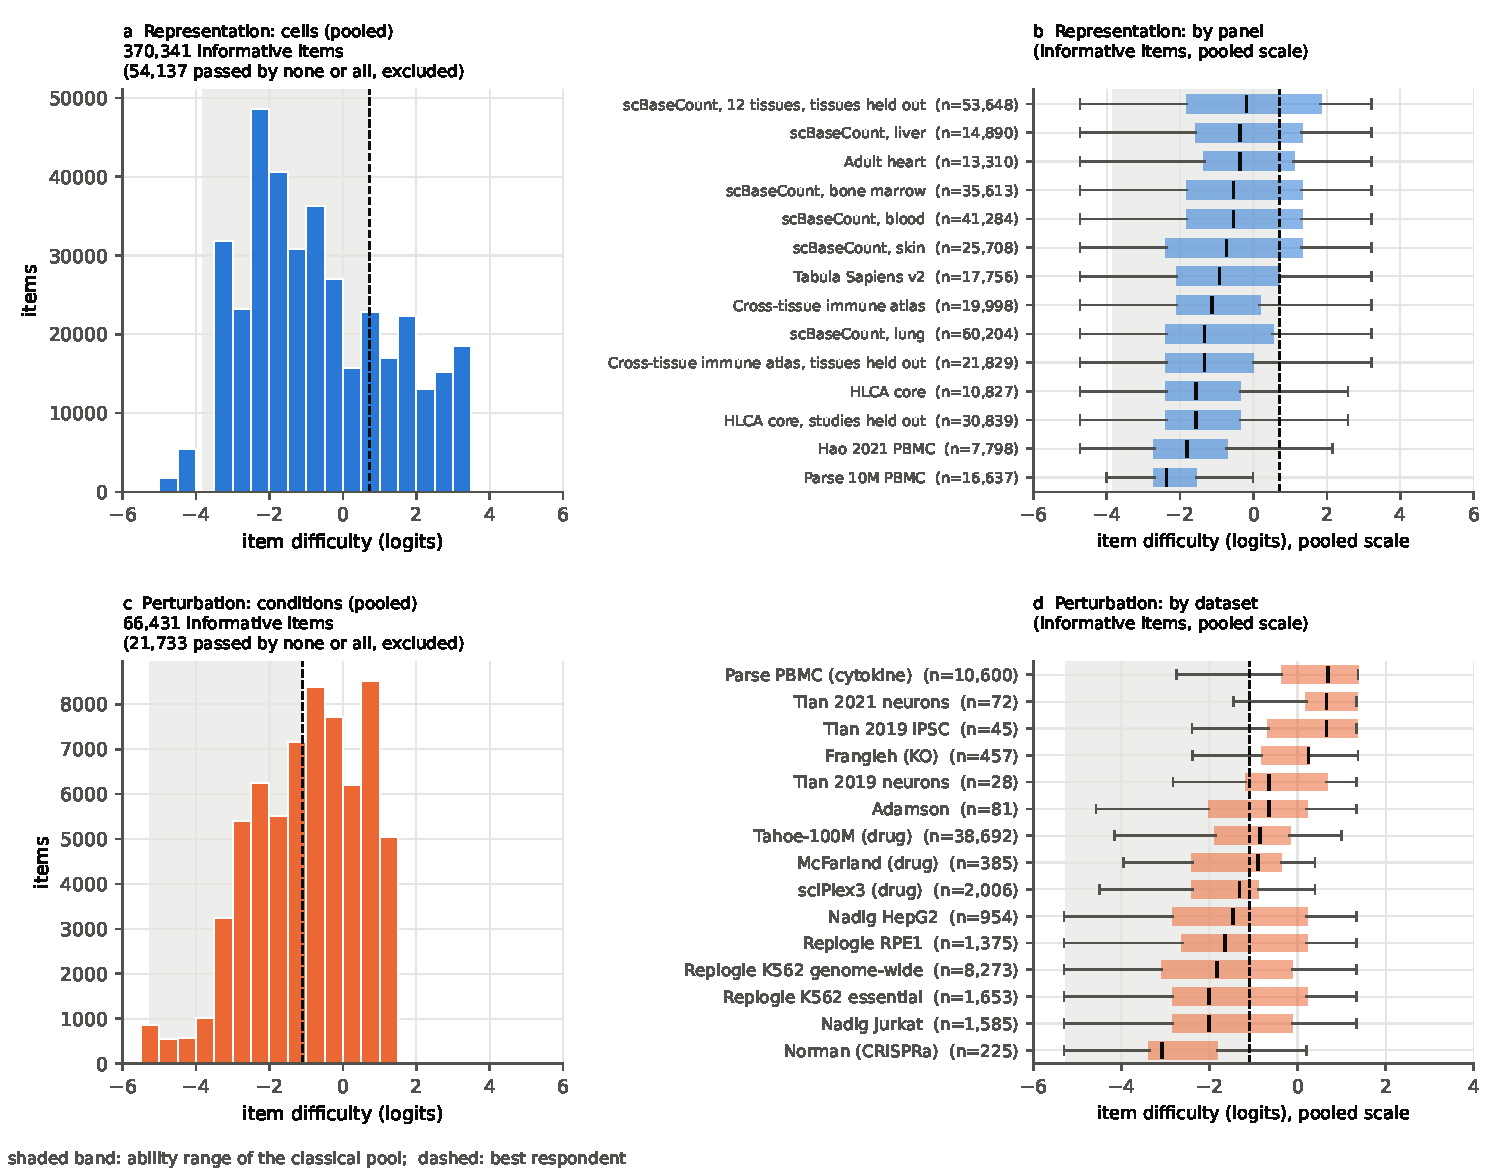
\includegraphics[width=0.96\textwidth]{fig_difficulty.pdf}
\caption{Item difficulty. (a) Representation items, one per cell, on the pooled scale of
all fourteen panels. (b) The same items by panel. (c) Perturbation conditions pooled across
datasets and (d) the same conditions by dataset. Boxes span the interquartile range and
whiskers the 5th to 95th percentile. The shaded band is the ability range of the simple
models and the dashed line the best of them. An item is informative when at least one model
passes it and at least one fails it.}
\label{fig:difficulty}
\end{figure}

% ---------------------------------------------------------------------------
\section{Method: Estimating Difficulty and Ability}
\label{sec:method}

\Cref{fig:pipeline} summarizes the pipeline. Both components end in the same object, a
pass/fail matrix with one row per model and one column per item, and the same fit turns
that matrix into abilities and difficulties.

\begin{figure}[t]
\centering
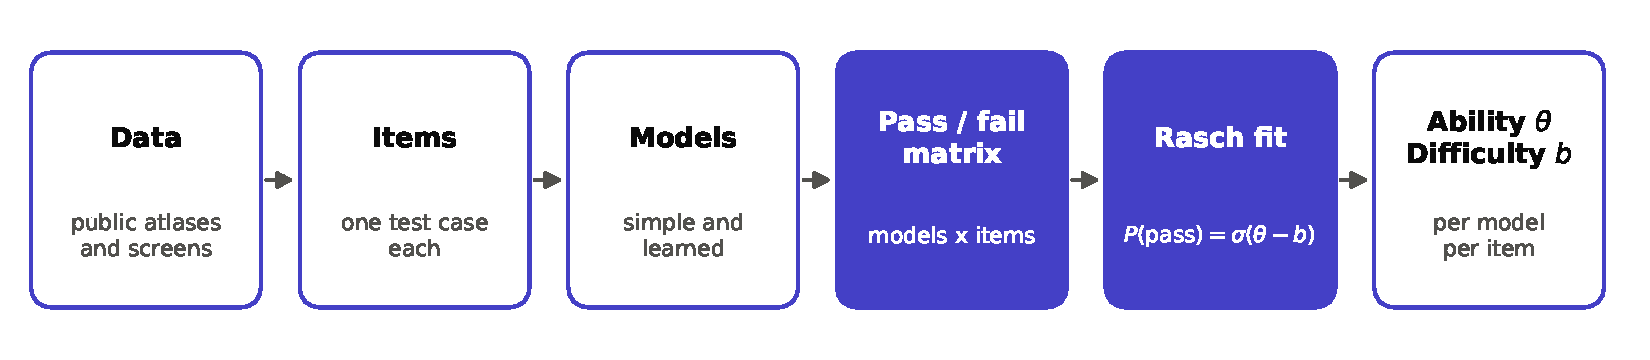
\includegraphics[width=\textwidth]{fig_pipeline.pdf}
\caption{From raw data to a difficulty scale. The same pipeline applies to both components:
items are built from public data, every model answers every item, the answers form a
pass/fail matrix, and one fit converts the matrix into an ability for every model and a
difficulty for every item.}
\label{fig:pipeline}
\end{figure}

\subsection{Models, items, and ability}
\label{sec:model}

There are $M$ models, indexed by $j\in\{1,\dots,M\}$; model $j$ has an ability
$\theta_j\in\mathbb{R}$. Items are drawn from a universe $\mathcal{U}$; item $i$ has a
difficulty $b_i\in\mathbb{R}$. We use the one-parameter Rasch model: model $j$ passes item
$i$ with probability
\begin{equation}
P(U_{ij}=1)=\sigma(\theta_j-b_i),\qquad \sigma(z)=\frac{1}{1+e^{-z}},
\label{eq:rasch}
\end{equation}
so an item is fully described by its difficulty. The unit of the scale is a logit: one unit
of extra ability multiplies the odds of passing any item by $e\approx2.7$. The information
a single item carries about a model's ability is
\begin{equation}
I_b(\theta)=\sigma(\theta-b)\bigl(1-\sigma(\theta-b)\bigr)\le\tfrac14,
\label{eq:info}
\end{equation}
which is largest when the difficulty matches the ability and falls off like
$e^{-|\theta-b|}$ on either side: an item is most telling for models near its own level,
and nearly useless for models that almost always pass or almost always fail it. Given a
model's answers to items of known difficulty, its ability is the penalized maximum
likelihood estimate
\begin{equation}
\hat\theta_j=\arg\max_{\theta}\sum_i\Bigl[U_{ij}\log\sigma(\theta-b_i)
+(1-U_{ij})\log\bigl(1-\sigma(\theta-b_i)\bigr)\Bigr]-\frac{\theta^2}{2\tau^2},
\label{eq:fit}
\end{equation}
which has a unique solution. The companion paper \citep{companion} builds on
\cref{eq:rasch,eq:info,eq:fit} to show how a bank of items should be maintained as models
improve; here we use them to build the bank.

\subsection{From benchmark outputs to a pass/fail matrix}
\label{sec:responses}

\begin{enumerate}[leftmargin=1.5em,itemsep=2pt]
\item \textbf{Build items.} Component A: select the test panels of \Cref{sec:data} and
record each cell's annotated type. Component B: map every screen to the common schema,
filter cells, and compute each condition's response as the mean log-normalized expression
of its cells minus that of its matched control cells.
\item \textbf{Run every model on every item.} Component A: for each panel, fit the
embedding on its training cells, embed both sides, train the fixed classifier on the
training embedding, and predict the test cells. Component B: for each of five folds, fit
the model on the training conditions and predict the held-out ones, so that every
condition receives exactly one out-of-fold prediction per model.
\item \textbf{Score and binarize.} Component A: $U_{ij}=1$ if the predicted type equals the
annotated type. Component B: compute the Pearson correlation between the predicted and
measured response over the 2,000 most variable genes, and set $U_{ij}=1$ if it exceeds the
mean shift's correlation on the same item. The continuous scores are stored as well.
\item \textbf{Assemble the matrix.} Rows are models, columns are items, entries are
$U_{ij}$; a pair that was not run, for example low-rank completion on a single-context
screen, is left missing and contributes nothing to the likelihood. Items from different
panels or screens are kept distinct even when the same cell appears in two panels under
two splits.
\end{enumerate}

\subsection{Fitting difficulties and abilities}
\label{sec:fitting}

All abilities and difficulties are estimated at once from the matrix. The objective is
the log-likelihood of \cref{eq:rasch} summed over observed pairs, with a Gaussian prior
$\theta_j\sim\mathcal{N}(0,\tau^2)$ on abilities, $\tau=3$, and a weaker one
$b_i\sim\mathcal{N}(0,\tau_b^2)$ on difficulties, $\tau_b=4$. The prior on difficulties
does two jobs: it fixes the location of the scale, which the likelihood alone leaves free
because only differences $\theta_j-b_i$ enter \cref{eq:rasch}, and it keeps items that
every model passes or every model fails at a finite value instead of sending them to
$\pm\infty$. Such items are flagged and excluded from the summaries in
\Cref{sec:data,sec:eval}; they carry no information about the current pool.

We maximize by alternating Newton steps: holding difficulties fixed, every ability is
updated by one Newton step of its own one-dimensional concave problem; holding abilities
fixed, every difficulty is updated likewise; the two sweeps repeat until the largest
change falls below $10^{-6}$, which takes a few hundred sweeps and eight minutes of compute
for the 424,478 annotation items. The same code path handles the stratum-level fit for
component A, where an item is a stratum answered $k$ times correctly out of $n$ cells, by
replacing each Bernoulli term with a binomial one. Each component is fit on one pooled
scale: all fourteen panels together, and all fifteen screens together, linked through the
models, which answer every panel and every screen under the same name.

Two checks validate the fit. On synthetic data generated from \cref{eq:rasch} with 80
models and 2,000 items at 30\% missingness, the recovered abilities correlate 0.998 with
the truth and the difficulties 0.969. On real data, the floors, which are random
embeddings, random shifts and predicting no change, must come out at the bottom of the
scale, and every capacity ladder must come out in order; \Cref{sec:eval} confirms this
before any other reading of the scale is made.

\paragraph{What the scale does and does not say.}
Ability is relative to the pool that defined the difficulties: a value of $0.69$ for
PCA-128D means it passes a typical item of this bank with probability $\sigma(0.69-b)$,
not that it is good in an absolute sense. Difficulty is likewise relative to the models: an
item is hard because these methods fail it. Both are comparable across models within a
component and, with the caveats in \Cref{sec:data}, across datasets within a component;
they are not comparable between the two components, which are fit separately.

% ---------------------------------------------------------------------------
\section{Model Evaluation}
\label{sec:eval}

A difficulty scale is only as trustworthy as the models that define it. We calibrate with
methods that are cheap, transparent, and cannot have seen the test data during
pretraining. Within each family we vary one capacity setting so that abilities spread out
in a known order, and we include several families so that items which one family passes
and another fails become visible. Floors pin the bottom of the scale. Pretrained
foundation models are placed on the scale afterwards; this is the only order in which
their abilities can be read separately from their exposure to the test data.

\subsection{The model pool}
\label{sec:pool}

\Cref{tab:pool} lists every model. All component A models see the same input:
log-normalized counts on the 2,000 most variable genes of the training panel, standardized
per gene; each is fit on training cells only and then applied to test cells, so test cells
never shape an embedding. This rules out UMAP and t-SNE, which have no out-of-sample map.
Component B models predict a condition's response from two inputs: the responses of the
training conditions, and a feature vector for the condition. Genetic items are represented
by a 64-dimensional embedding of the target gene learned from control cells only, with
genes as rows, cells as columns and principal components across cells; compounds by Morgan
fingerprints of their chemical structure \citep{morgan} together with the dose and a
one-hot context indicator. Cytokines have neither a target gene nor a structure in their
source files, so Parse items carry one-hot indicators of the cytokine and of the context;
with these features the regression models become additive models of a cytokine effect and
a context effect, and the nearest-neighbour model becomes the average response of the same
cytokine in other contexts.

\begin{table}[t]
\centering
\caption{The model pool. Each row is one family; the setting varied within the family is
given in the last column. For component B, $d$ is the number of principal components of
the training responses that a model predicts before decoding back to genes, and the kernel
width is a multiple of the median pairwise distance between training conditions. Learned
models are listed last; they are placed on the scale the simple models define.}
\label{tab:pool}
\footnotesize
\begin{tabularx}{\textwidth}{@{}lXl@{}}
\toprule
Model & What it does & Settings \\
\midrule
\multicolumn{3}{@{}l}{\emph{Component A: embeddings of a cell, followed by the same fixed classifier}} \\
PCA-$k$D & top-$k$ principal components & $k\in\{4,8,16,32,64,128,256\}$ \\
Random projection-$k$D & Gaussian random projection to $k$ dimensions & $k\in\{8,32,128\}$, 2 seeds \\
Nystr\"om-$k$D & RBF kernel features on PCA-50D & $k\in\{64,256\}$, kernel width 0.5 or 2 \\
NMF-$k$D & non-negative matrix factorization & $k\in\{16,64\}$ \\
ICA-$k$D & independent components of PCA-$k$D & $k\in\{16,64\}$ \\
GMM-$k$ memberships & soft cluster memberships from a Gaussian mixture on PCA-50D & $k\in\{10,30,100\}$ \\
Depth only & two numbers, log total counts and log detected genes; a floor & \\
Random-32D & i.i.d.\ Gaussian features; a floor & 2 seeds \\
scVI-$k$D & variational autoencoder for counts \citep{scvi}, with and without the panel's context as the batch variable & $k\in\{10,30\}$ \\
\midrule
\multicolumn{3}{@{}l}{\emph{Component B: prediction of a condition's response}} \\
No change & predicts zero response; a floor & \\
Random shift & the response of a random training condition; a floor & 2 seeds \\
Mean shift & the average response of the training conditions in that context; defines the pass rule & \\
Mean shift + on-target change & mean shift with the target gene forced down for CRISPRi and knockout or up for CRISPRa & \\
KNN (K=$k$) & average response of the $k$ nearest training conditions in feature space & $k\in\{1,5,20\}$ \\
Ridge ($d$, $\lambda$) & ridge regression from features to the top-$d$ components of the responses & $d\in\{10,50\}$, $\lambda\in\{1,100\}$ \\
PCA regression-$k$D & ridge to the top-$k$ components with a fixed penalty; the capacity ladder of this component & $k\in\{2,5,10,20,50,100,200\}$ \\
Gaussian process (kernel width) & Gaussian-process regression with an RBF kernel on features, to the top-50 components & kernel width 0.5 or 2 \\
Training-fraction ladder & ridge and KNN trained on a random 30\% or 10\% of the training conditions & 2 fractions \\
Low-rank completion & soft-impute of the perturbation-by-context response matrix; multi-context screens only & rank $\in\{2,5,10\}$ \\
scGen & variational autoencoder with latent arithmetic \citep{scgen}; unseen-context setting only & \\
\bottomrule
\end{tabularx}
\end{table}

\paragraph{Splits.}
Perturbation models are evaluated out of fold: perturbations are divided into five folds,
each model is trained on four and predicts the fifth, and every condition therefore
receives a prediction from a model that never saw its perturbation. Screens with several
contexts are additionally split over perturbation and context pairs, so that a
perturbation seen in some contexts must be predicted in a new one. Representation models
are fit on each panel's training cells and scored on that panel's held-out donors,
studies, or tissues. All models share the same folds, panels, classifier, and metrics.

\paragraph{Fit.}
Abilities and difficulties are estimated as in \Cref{sec:fitting}. For cells we report a
cell-level fit and a stratum-level binomial fit; the two order the models identically.

\begin{figure}[t]
\centering
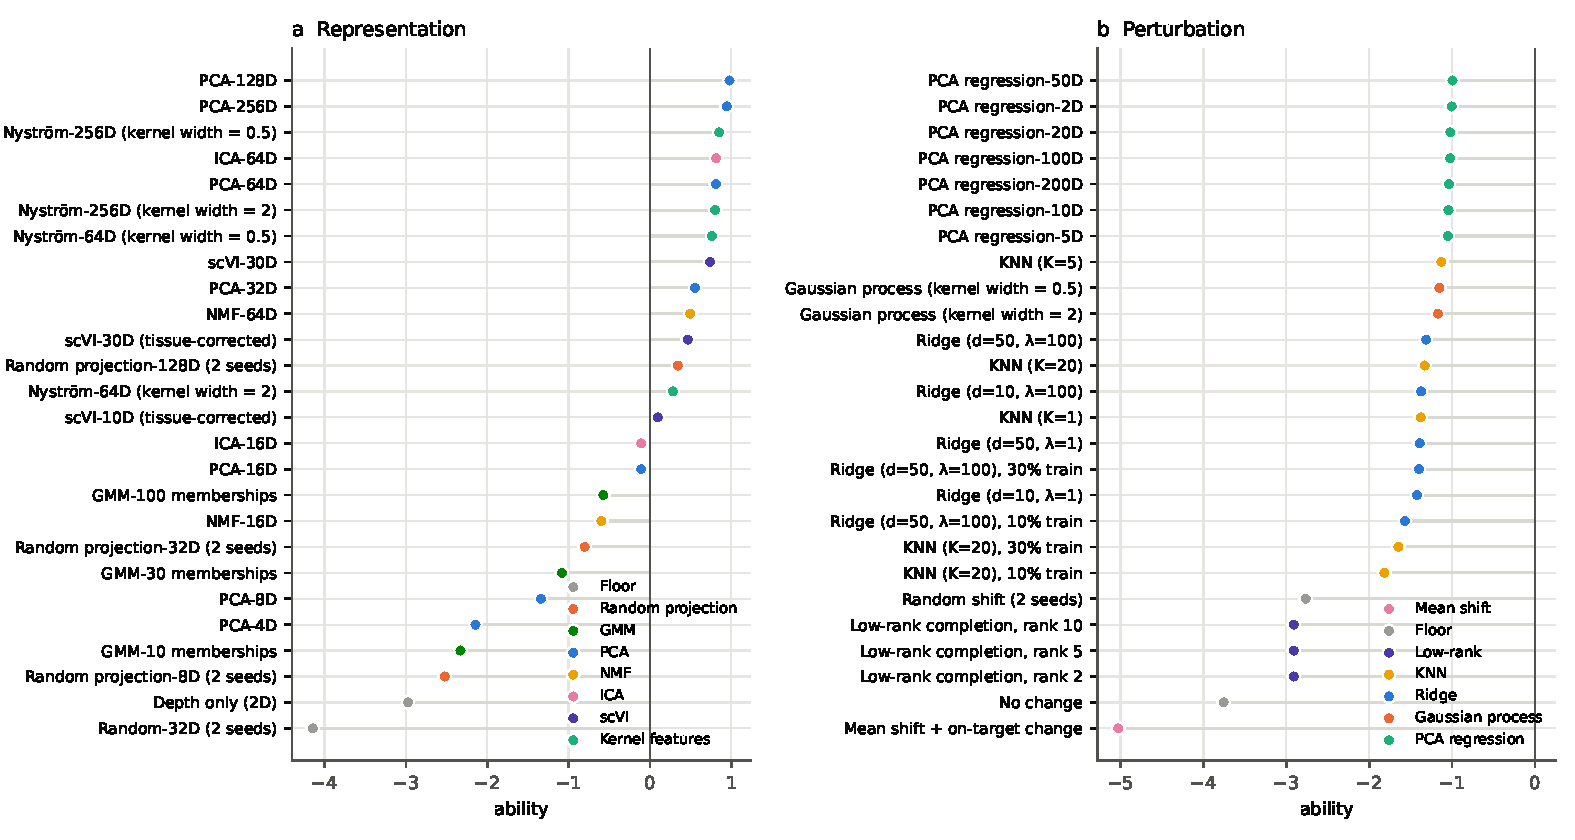
\includegraphics[width=\textwidth]{fig_abilities.pdf}
\caption{Abilities of the model pool. (a) Representation models on the pooled cell-level
scale of all fourteen panels, 424,478 items. (b) Perturbation models on the pooled scale
of all fifteen screens, 88,164 conditions. Colour marks the family; the two seeds of a
stochastic model are averaged. The mean shift defines the pass rule and therefore has no
ability of its own. The full tables, with plain accuracy alongside ability for component
A, are in \Cref{app:tables}.}
\label{fig:abilities}
\end{figure}

\subsection{Results}
\label{sec:results}

\Cref{fig:abilities}a gives the representation abilities on the pooled scale of all
fourteen panels. The best model is Nystr\"om-256D with kernel width 0.5 at $0.72$;
tissue-corrected scVI-30D is at $0.72$, scVI-30D without batch correction at $0.71$ and
PCA-128D at $0.69$, so the top four lie within $0.03$ of one another. PCA-256D, Nystr\"om-64D,
ICA-64D and PCA-64D follow at $0.66$ to $0.67$, then Nystr\"om-256D with kernel width 2 at
$0.62$ and PCA-32D at $0.53$. The next group is Nystr\"om-64D with width 2 at $0.42$, NMF-64D
at $0.41$ and tissue-corrected scVI-10D at $0.37$. PCA-16D and ICA-16D are at $0.11$, the
128-dimensional random projections at $-0.08$, GMM-100 at $-0.18$ and NMF-16D at $-0.37$.
Below zero by more than half a unit are PCA-8D ($-0.67$), GMM-30 ($-0.68$), the
32-dimensional random projections ($-1.30$), PCA-4D ($-1.50$), GMM-10 ($-1.88$) and the
8-dimensional random projections ($-2.70$); the depth-only floor is at $-3.14$ and the
random embeddings at $-3.83$. Plain accuracy is 0.618 for the best model and 0.615 for
PCA-128D; the eight best models are within one accuracy point of one another
(\Cref{tab:abilA}). Ability rises with dimension in every family: PCA from $-1.50$ at 4
dimensions to $0.69$ at 128, with 256 at $0.67$; random projections from $-2.70$ at 8 to
$-0.08$ at 128, which is 0.8 to 2.0 below PCA at the same dimension.

Fit panel by panel, the best model is scVI-30D on five panels: Hao PBMC ($3.57$), the HLCA
with studies held out ($2.82$), the immune atlas with tissues held out ($2.17$), scBaseCount
blood ($0.53$) and scBaseCount bone marrow ($0.31$). It is Nystr\"om-256D on six: Parse
($3.41$), the immune atlas with donors held out ($2.01$), scBaseCount lung ($1.44$, level with
PCA-128D), adult heart ($0.63$), scBaseCount skin ($0.41$) and scBaseCount liver ($-0.03$).
It is PCA-128D on the HLCA with donors held out ($2.69$) and on Tabula Sapiens ($0.98$), and
Nystr\"om-64D on the twelve-tissue scBaseCount panel ($-1.15$). scVI-30D is below PCA-128D by
$0.24$ on Tabula Sapiens, by $0.12$ on the donor-held-out HLCA, by $0.18$ on the
donor-held-out immune atlas, by $0.30$ on scBaseCount lung and by $0.13$ on the
twelve-tissue panel, and above it by $0.39$ on scBaseCount blood, $0.26$ on bone marrow and
$0.08$ on skin. On Tabula Sapiens, plain accuracy rises from 0.606 at PCA-32D to 0.654 at
PCA-128D while ability rises from $0.55$ to $0.98$ (\Cref{tab:abilA_ts2}). The top raw
accuracy per panel is 0.61 to 0.89 on the eight curated panels and 0.39 to 0.70 on the six
scBaseCount panels; between the 60-sample and 200-sample versions of the scBaseCount blood
panel, scVI-30D's accuracy rose from 0.50 to 0.60 and the best classical model's from 0.46 to
0.56, while on lung, skin and liver the top accuracy changed by less than 0.02.

\Cref{fig:abilities}b gives the perturbation abilities on the pooled scale of all fifteen
screens in the unseen-perturbation split. The best model is KNN with $K=20$ at $-1.10$,
followed by KNN with $K=5$ at $-1.19$, PCA regression with 200 components at $-1.34$, the
Gaussian processes at $-1.38$ and $-1.42$, PCA regression-100D at $-1.52$ and KNN with $K=1$
at $-1.54$. The ridge models lie between $-1.58$ and $-1.71$ and the PCA-regression ladder
rises from $-1.73$ at 5 components to $-1.34$ at 200. The training-fraction ladders are in
order: ridge at $-1.58$ on the full training set, $-1.63$ at 30\% and $-1.76$ at 10\%; KNN
($K=20$) at $-1.10$, $-1.63$ and $-2.00$. Below them are the random shifts at $-2.93$,
low-rank completion at $-2.97$, no change at $-3.88$ and the mean shift with the on-target
change at $-5.27$. Ranked by raw Pearson correlation instead, the best model in eight of the
fifteen screens, Tahoe-100M and Parse among them, is the mean shift or its on-target
variant; the exception with the widest margin is Norman, where the Gaussian process reaches
0.69 against 0.49 for the mean shift.

In the unseen-combination split, where a perturbation has been seen in other contexts and
the context with other perturbations, the picture differs. On Tahoe-100M, low-rank
completion reaches a raw correlation of 0.75 and KNN ($K=20$) 0.73 against 0.42 for the
mean shift, which ranks 18th of 21 models, and 169 of 53,972 conditions are passed by no
model. On Parse, PCA regression with 200 components on one-hot features reaches 0.50
against 0.36 for the mean shift and passes 87\% of items, with ability $3.74$ on that screen;
low-rank completion reaches 0.45 and passes 59\%; 719 of 13,967 conditions are passed by
no model. In Parse's unseen-cytokine split, KNN ($K=20$) passes 47\% of items and every other
model fewer than 17\%, none exceeds the mean shift's raw correlation of 0.36 on average, and
3,367 conditions are passed by no model. scGen was run in this split on the three screens
of \Cref{tab:scgen}: on McFarland it passes 81\% of items with ability $+2.75$, first of
nine models, with a raw correlation of 0.53 against 0.32 for the mean shift; on sciPlex3 it
is fourth of nine at $-1.76$ with 0.13 against 0.26; on Frangieh tenth of 22 at $-2.77$ with
0.18 against 0.32. Because it is run per screen in this split, it is not on the pooled
scale of \Cref{fig:abilities}b.

\begin{table}[t]
\centering
\caption{scGen in the unseen-combination split. Raw is the mean Pearson correlation on the
2,000 most variable genes, next to the mean shift's value. Rank is among the models that
ran on that screen.}
\label{tab:scgen}
\small
\begin{tabular}{@{}lrrrrl@{}}
\toprule
Screen & Contexts & Raw scGen & Raw mean shift & Ability and rank & Best model \\
\midrule
McFarland 2020 & 196 & 0.53 & 0.32 & $+2.75$, 1 of 9 & scGen \\
sciPlex3, Srivatsan 2020 & 3 & 0.13 & 0.26 & $-1.76$, 4 of 9 & low-rank, rank 10 \\
Frangieh 2021 & 3 & 0.18 & 0.32 & $-2.77$, 10 of 22 & low-rank, rank 5 \\
\bottomrule
\end{tabular}
\end{table}

\Cref{fig:retire} gives the fraction of items that are already uninformative for the
evaluated models: an item is too easy at threshold $t$ when every model other than the
floors passes it with probability at least $t$, and too hard when every one fails it with
probability at least $t$. At $t=0.75$, 0.3\% of cell items and 0.1\% of conditions are too
easy and 24\% and 47\% are too hard; at $t=0.95$ the too-hard fractions are 12.5\% and 25\%,
which are the items no model passes. A model one logit above the best current one would
move 45\% of the cell items and 9\% of the conditions into the too-easy class at $t=0.95$;
the companion paper \citep{companion} relates this rate to the rate at which new items must
be added.

\begin{figure}[t]
\centering
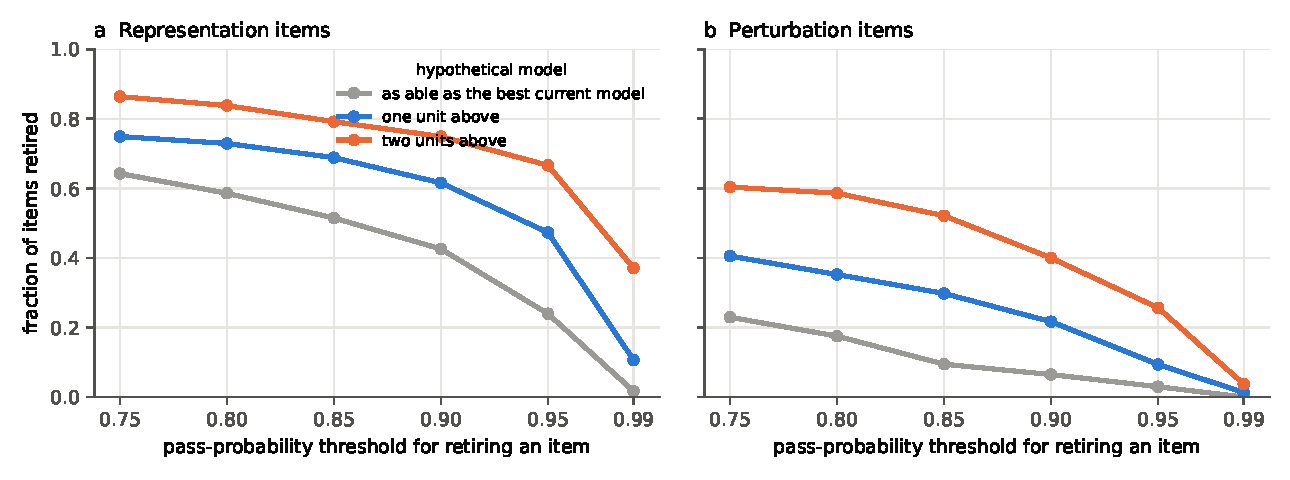
\includegraphics[width=0.9\textwidth]{fig_retire.pdf}
\caption{Fraction of items that are uninformative for the evaluated models, as a function of
the probability threshold $t$. An item is too easy when every model other than the floors
passes it with probability at least $t$, and too hard when every one fails it with
probability at least $t$; items passed by none or by all models count in the respective
class. (a) Representation items. (b) Perturbation items.}
\label{fig:retire}
\end{figure}

The pool has about 30 models per component. The pooled scales carry a between-dataset
spread of 1.9 units across annotation panels and 3.2 across perturbation screens. The
compounds in sciPlex3 and McFarland lack chemical structures in their source files and the
cytokines in Parse lack any descriptor, so those screens run in the unseen-combination
split and, for Parse, as a floor in the unseen-perturbation split. No pretrained foundation
model has yet been placed on either scale.

% ---------------------------------------------------------------------------
\section{Conclusion}
\label{sec:conclusion}

We have built a benchmark for virtual cell models in which every test case has a measured
difficulty, assembled from about 110 million cells across fourteen annotation panels and
fifteen perturbation screens, and calibrated it with a pool of simple models. The scale
spans about six logits in each component, its capacity ladders are ordered, and the
abilities of every evaluated model are reported on it alongside plain accuracy. Because the
scale is anchored to methods that cannot have memorized the test data, it is ready to
receive pretrained foundation models next, and because it records which items each model
passes, it tells us how fast new hard items must be written to keep the benchmark alive.

\bibliographystyle{acl_natbib}
\bibliography{benchmark}

\beginappendix
\section{Ability tables}
\label{app:tables}

\begin{table}[h]
\centering
\caption{Representation models on the pooled cell-level scale of all fourteen panels,
424,478 items: ability and plain accuracy, which is the fraction of test cells labelled
correctly.}
\label{tab:abilA}
\small
\begin{tabular}{@{}lrr@{}}
\toprule
Model & Ability & Accuracy \\
\midrule
PCA-128D & 0.98 & 0.654 \\
PCA-256D & 0.94 & 0.650 \\
Nyström-256D (kernel width = 0.5) & 0.85 & 0.640 \\
ICA-64D & 0.81 & 0.636 \\
PCA-64D & 0.81 & 0.635 \\
Nyström-256D (kernel width = 2) & 0.80 & 0.634 \\
Nyström-64D (kernel width = 0.5) & 0.76 & 0.630 \\
scVI-30D & 0.74 & 0.627 \\
PCA-32D & 0.55 & 0.606 \\
NMF-64D & 0.49 & 0.599 \\
scVI-30D (tissue-corrected) & 0.47 & 0.596 \\
Random projection-128D (seed 0) & 0.35 & 0.582 \\
Random projection-128D (seed 1) & 0.34 & 0.581 \\
Nyström-64D (kernel width = 2) & 0.28 & 0.574 \\
scVI-10D (tissue-corrected) & 0.10 & 0.552 \\
ICA-16D & -0.11 & 0.526 \\
PCA-16D & -0.11 & 0.526 \\
GMM-100 memberships & -0.57 & 0.464 \\
NMF-16D & -0.60 & 0.461 \\
Random projection-32D (seed 1) & -0.75 & 0.440 \\
Random projection-32D (seed 0) & -0.85 & 0.426 \\
GMM-30 memberships & -1.08 & 0.394 \\
PCA-8D & -1.34 & 0.359 \\
PCA-4D & -2.14 & 0.251 \\
GMM-10 memberships & -2.33 & 0.228 \\
Random projection-8D (seed 0) & -2.47 & 0.211 \\
Random projection-8D (seed 1) & -2.57 & 0.199 \\
Depth only (2D) & -2.97 & 0.156 \\
Random-32D (seed 1) & -4.14 & 0.066 \\
Random-32D (seed 0) & -4.14 & 0.066 \\
\bottomrule
\end{tabular}

\end{table}

\begin{table}[h]
\centering
\caption{Representation models on the Tabula Sapiens v2 panel alone, 20,026 items, the
panel on which the pool was first calibrated.}
\label{tab:abilA_ts2}
\small
\begin{tabular}{@{}lrr@{}}
\toprule
Model & Ability & Accuracy \\
\midrule
PCA-128D & 0.98 & 0.654 \\
PCA-256D & 0.94 & 0.650 \\
Nyström-256D (kernel width = 0.5) & 0.85 & 0.640 \\
ICA-64D & 0.81 & 0.636 \\
PCA-64D & 0.81 & 0.635 \\
Nyström-256D (kernel width = 2) & 0.80 & 0.634 \\
Nyström-64D (kernel width = 0.5) & 0.76 & 0.630 \\
scVI-30D & 0.74 & 0.627 \\
PCA-32D & 0.55 & 0.606 \\
NMF-64D & 0.49 & 0.599 \\
scVI-30D (tissue-corrected) & 0.47 & 0.596 \\
Random projection-128D (seed 0) & 0.35 & 0.582 \\
Random projection-128D (seed 1) & 0.34 & 0.581 \\
Nyström-64D (kernel width = 2) & 0.28 & 0.574 \\
scVI-10D (tissue-corrected) & 0.10 & 0.552 \\
ICA-16D & -0.11 & 0.526 \\
PCA-16D & -0.11 & 0.526 \\
GMM-100 memberships & -0.57 & 0.464 \\
NMF-16D & -0.60 & 0.461 \\
Random projection-32D (seed 1) & -0.75 & 0.440 \\
Random projection-32D (seed 0) & -0.85 & 0.426 \\
GMM-30 memberships & -1.08 & 0.394 \\
PCA-8D & -1.34 & 0.359 \\
PCA-4D & -2.14 & 0.251 \\
GMM-10 memberships & -2.33 & 0.228 \\
Random projection-8D (seed 0) & -2.47 & 0.211 \\
Random projection-8D (seed 1) & -2.57 & 0.199 \\
Depth only (2D) & -2.97 & 0.156 \\
Random-32D (seed 1) & -4.14 & 0.066 \\
Random-32D (seed 0) & -4.14 & 0.066 \\
\bottomrule
\end{tabular}

\end{table}

\begin{table}[h]
\centering
\caption{Perturbation models on the pooled scale of all fifteen screens, 88,164 conditions.
Low-rank completion ran only on multi-context screens and, in the unseen-perturbation
setting, can only fall back to the context mean for a perturbation it has never seen.}
\small
\begin{tabular}{@{}lr@{}}
\toprule
Model & Ability \\
\midrule
KNN (K=20) & -1.10 \\
KNN (K=5) & -1.19 \\
PCA regression-200D & -1.34 \\
Gaussian process (kernel width = 0.5) & -1.38 \\
Gaussian process (kernel width = 2) & -1.42 \\
PCA regression-100D & -1.52 \\
KNN (K=1) & -1.54 \\
Ridge (d=50, $\lambda$=100) & -1.58 \\
PCA regression-50D & -1.58 \\
KNN (K=20), 30\% train & -1.62 \\
Ridge (d=50, $\lambda$=100), 30\% train & -1.63 \\
Ridge (d=50, $\lambda$=1) & -1.65 \\
PCA regression-20D & -1.66 \\
Ridge (d=10, $\lambda$=100) & -1.67 \\
Ridge (d=10, $\lambda$=1) & -1.71 \\
PCA regression-10D & -1.71 \\
PCA regression-2D & -1.72 \\
PCA regression-5D & -1.73 \\
Ridge (d=50, $\lambda$=100), 10\% train & -1.76 \\
KNN (K=20), 10\% train & -2.00 \\
Random shift (seed 0) & -2.93 \\
Random shift (seed 1) & -2.93 \\
Low-rank completion, rank 10 & -2.97 \\
Low-rank completion, rank 5 & -2.97 \\
Low-rank completion, rank 2 & -2.97 \\
No change & -3.88 \\
Mean shift + on-target change & -5.27 \\
\bottomrule
\end{tabular}

\end{table}

\section{Implementation details}
\label{app:impl}

\begin{table}[h]
\centering
\caption{Representation panels in full. Held out is the unit whose members form the test
items and N held out counts them: donors, public samples, studies or tissues. Contexts are
the tissues or studies represented among the items; strata are context, cell type and donor
combinations.}
\label{tab:compA_full}
\scriptsize
\setlength{\tabcolsep}{4pt}
\begin{tabular}{@{}lrrrrrrr@{}}
\toprule
Panel & Held out & N held out & Contexts & Cell types & Train cells & Items & Strata \\
\midrule
Tabula Sapiens v2 & donors & 2 & 22 & 102 & 146,800 & 20,026 & 433 \\
Hao 2021 PBMC & donors & 3 & 3 & 24 & 42,441 & 7,999 & 171 \\
Adult heart & donors & 5 & 4 & 59 & 81,001 & 14,396 & 315 \\
HLCA core & donors & 11 & 11 & 52 & 134,615 & 11,389 & 247 \\
HLCA core & studies & 3 & 3 & 51 & 85,476 & 32,221 & 724 \\
Cross-tissue immune atlas & donors & 6 & 16 & 41 & 66,684 & 20,548 & 474 \\
Cross-tissue immune atlas & tissues & 5 & 5 & 38 & 59,565 & 23,038 & 521 \\
Parse 10M PBMC & donors & 5 & 2 & 18 & 45,948 & 16,811 & 176 \\
scBaseCount, lung & samples & 70 & 1 & 25 & 145,543 & 64,635 & 883 \\
scBaseCount, skin & samples & 35 & 1 & 15 & 68,112 & 28,812 & 346 \\
scBaseCount, bone marrow & samples & 62 & 1 & 20 & 104,777 & 41,262 & 513 \\
scBaseCount, liver & samples & 29 & 1 & 19 & 51,432 & 17,559 & 227 \\
scBaseCount, blood & samples & 80 & 1 & 14 & 129,019 & 46,625 & 578 \\
scBaseCount, 12 tissues & tissues & 5 & 5 & 22 & 180,127 & 79,157 & 979 \\
\midrule
Total & & & & 299 & 1,341,540 & 424,478 & 6,587 \\
\bottomrule
\end{tabular}

\end{table}

\section{The Tabula Sapiens panel by tissue}
\label{app:ts2}

\begin{table}[h]
\centering
\caption{Tabula Sapiens v2 panel by tissue. Donors and cell types count the whole panel;
training cells are the classifier's training set; items are the scored test cells and
strata their tissue, cell type and donor combinations. Tissues are ordered by item count.
Because the split is by donor, six tissues whose donors all fall on the training side
contribute training cells but no items, and Testis, with a single donor on the test side,
contributes items but no training cells.}
\label{tab:compA_ts2}
\footnotesize
\begin{tabular}{@{}lrrrrr@{}}
\toprule
Tissue & Donors & Cell types & Training cells & Items & Strata \\
\midrule
Small Intestine & 5 & 31 & 5,684 & 1,800 & 40 \\
Spleen & 6 & 21 & 10,604 & 1,326 & 28 \\
Fat & 6 & 20 & 5,897 & 1,234 & 26 \\
Stomach & 3 & 18 & 1,252 & 1,232 & 26 \\
Large Intestine & 5 & 25 & 4,785 & 1,228 & 26 \\
Tongue & 4 & 20 & 3,040 & 1,226 & 26 \\
Lung & 4 & 28 & 10,472 & 1,220 & 25 \\
Thymus & 5 & 25 & 9,098 & 1,219 & 29 \\
Bladder & 6 & 21 & 8,776 & 1,140 & 25 \\
Lymph Node & 6 & 19 & 9,119 & 1,039 & 22 \\
Heart & 5 & 15 & 2,618 & 1,026 & 22 \\
Muscle & 5 & 22 & 5,394 & 999 & 21 \\
Bone Marrow & 6 & 20 & 7,737 & 916 & 21 \\
Vasculature & 4 & 20 & 5,223 & 844 & 18 \\
Salivary Gland & 4 & 23 & 6,501 & 679 & 15 \\
Trachea & 5 & 20 & 4,086 & 621 & 15 \\
Prostate & 3 & 12 & 2,771 & 555 & 12 \\
Blood & 9 & 18 & 11,510 & 504 & 11 \\
Mammary & 2 & 12 & 1,837 & 498 & 10 \\
Ear & 2 & 9 & 298 & 300 & 6 \\
Ovary & 3 & 9 & 2,268 & 270 & 6 \\
Testis & 1 & 8 & 0 & 150 & 3 \\
Eye & 4 & 28 & 7,045 & 0 & 0 \\
Kidney & 1 & 10 & 1,371 & 0 & 0 \\
Liver & 4 & 20 & 7,673 & 0 & 0 \\
Pancreas & 2 & 14 & 2,594 & 0 & 0 \\
Skin & 4 & 14 & 4,954 & 0 & 0 \\
Uterus & 2 & 17 & 4,193 & 0 & 0 \\
\midrule
Total & 23 & 159 & 146,800 & 20,026 & 433 \\
\bottomrule
\end{tabular}

\end{table}

\end{document}
